\subsection{Sprachsynthese}

\subsubsection*{Benutzeroberfläche}

Erweiterung Inbox um T2S Icon. \\
Erweiterung Admin UI um Checkbox. \\
Zusätzlich Configuration Page mit preferences. \\

\subsubsection*{Konfiguration}

Erweiterung NotificationType um ein boolean Flag für isTextToSpeech.
Wenn Aktiviert, wird Benachrichtigung bei Empfang vorgelesen.

Weiter wird auf dem NotificationType ein Feld version hinzugefügt.
Damit soll die aktuelle Version des NotificationType verfolgt werden.
Wird eine Änderung am NotificationType persisteirt, wird die Version entsprechend angepasst.
Sowohl das Flag isTextToSpeech als auch das version Property werden neu beim Versenden von Benachrichtigungen mitgegeben.

Sprachsynthese kann auf Client Seite dekativiert werden.
Ist es deaktiviert, werden keine Benachrichtigungen vorgelesen.
Audio Signal, dass Benachrichtung empfangen wurde ertönt aber trotzdem.
Keine zusätzlichen Endpoints am Cloud Service nötig. \\

\begin{figure}[h]
    \centering
    \begin{minipage}[b]{0.75\textwidth}
        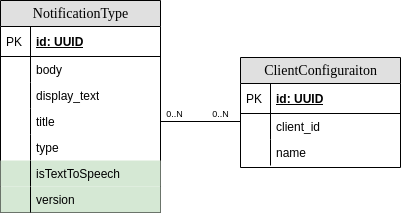
\includegraphics[width=\textwidth]{/home/joshua/FHNW/dev/IP6/IP6_Bachelorarbeit_Bericht_Cloudbasiertes_Praxisrufsystem/src/graphics/diagramms/erd_t2s_v01.drawio}
        \caption{ERD Ausschnitt - Konfiguration Sprachsynthese}
    \end{minipage}
\end{figure}

\clearpage

\subsection*{Anbindung Sprachsynthese Service}

Die Anbindung des Sprachsynthese Service erfolg zentral über den Cloud Service.
Dazu wird der Cloud Service um ein modul Speech erweitert.
Dieses Modul stellt einen Endpoint zur verfügung über den die Sprachdaten zu einer Benachrichtigung abgefragt werden können.
Einziger Parameter für diese Anfrage ist die technische Identifikation des Benachrichtigungstyps der relevanten Benachrichtigung.
Das Speech-Modul kann anhand dieser Identifikation den NotificationType beim Configuration-Modul abholen.
Dem NotificationType kann der Text entonmmen werden, der snytetisiert werden soll.
Dieser Text kann dann an den Sprachsynthese Service gesendet werden.
Das Resultat dieser Anfrage wird als Resultat der Abfrage vom Client zurückgegeben.

\lstinputlisting[caption=SpeechSynthesisController.java,language=java,label={lst:SpeechSynthesisController.java}]{listings/SpeechSynthesisController.java}

Auf Client seite kann dieser Endpunkt nun als Download angesprochen werden.

\lstinputlisting[caption=PraxisrufApi+Speech.swift,language=swift,label={lst:PraxisrufApi+Speech.swift}]{listings/PraxisrufApi+Speech.swift}

Um die Anbindung im Cloud Service vom konkreten Anbieter möglichst unabhängig zu machen, wird die Integration an den Speech Synthese Service über ein Interface abstrahiert.
Soll ein neuer Sprachsyntese Service angebunden werden, muss lediglich dieses Interface für den neuen Service implementiert werden und alles andere kann unberührt bleiben.

\clearpage

\lstinputlisting[caption=SpeechSynthesisService.java,language=java,label={lst:SpeechSynthesisService.java}]{listings/SpeechSynthesisService.java}

Für dieses Projekt wird AWS Polly verwendet.
Dementsprechend wird das SprachSyntheseService Interface für AWS Polly implementiert.
AWS Polly bietet einen Java SDK, welcher die Anbindung ermöglicht.
Dieser SDK bietet alle Klassen die für die Anbindung an AWS Polly nötig sind.
Da im Cloud Service Spring Boot verwendet wird, können die für die Verbindung nötigen Klassen mit einer Spring Config erstellt werden
und dann über Dependency Injection im AwsPollySpeechSynthesis Service verwendet werden.

\lstinputlisting[caption=AwsConfiguration.java,language=java,label={lst:AwsConfiguration.java}]{listings/AwsConfiguration.java}

In der Implementation des Services kann nun über den injezierten AmazonPollyClient eine Abfrage an den Speech Synthesis Service gesendet werden.

\clearpage

\subsection*{Laufzeitsicht}

Benachrichtigungen für welche Sprachsynthese aktiviert ist, sollen beim Empfang automatisch vorgelesen werden.
Dazu müssen die Sprachdaten geladen werden, wenn die Benachrichtigung empfangen werden.
Diese Daten können über den neuen Speech Endpoint des Cloud Services bezogen werden.
Die Informationen die dazu nötig sind, sind als Metadaten in der empfangenen Benachrichtigung vorhanden.

\begin{figure}[h]
    \centering
    \begin{minipage}[b]{0.9\textwidth}
        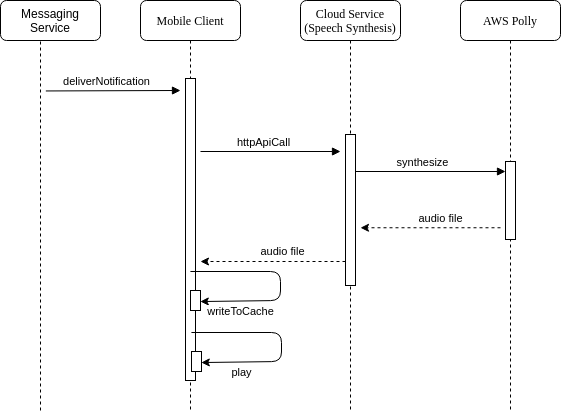
\includegraphics[width=\textwidth]{graphics/diagramms/Sequence_Speech_Synth_V01}
        \caption{Ablauf Benachrichtigung empfangen}
    \end{minipage}
\end{figure}

Wird eine Benachrichtigung empfangen, wird die Benachrichtigung auf dem Client als Push Notifikation angezeigt und an die Inbox übergeben.
Anschliessend prüft der Client ob die Sprachdaten für die Empfangene Benachrichtigung bereits lokal zur Verfügung stehen.
Dies wird gemacht in dem er überprüft ob es im Applikationsverzeichnis bereits eine MP3-Datei für den Empfangenen Benachrichtigungstyp
(NotificationType) in der Version der Empfangenen Benachrichtigung vorhanden ist.
Sind die Daten bereits lokal vorhanden, wird keine Abfrage an den Cloud Service gespielt sondern die lokal vorhandene Sprachdatei abgespielt.
Sind die Daten lokal nicht oder nur in einer anderen Version vorhanden, werden die Daten beim Cloudservice angefragt.
Sobald diese Daten geladen sind, werden sie in einer MP3 Datei mit Id und Version des Benachrichtigungstyps (NotificationType) gespeichert.

\clearpage
